%% ============================================================
\section{Design}\label{sec:design}
%% ============================================================

{\color{red}\textbf{Reto is currently working here.}}

\autoref{fig:validation-pipeline} shows the overview of our model validation pipeline.
The goal is to systematically validate the hardware model against real hardware. 
The validation pipeline consists of a test-case generator, a test execution harness, a trace validator. 
The input to the pipeline is a reduced hardware model that provides the basis for generating the test programs and trace validation.
Next, we elaborate on the purpose of each component in the validation pipeline.

\begin{figure*}[t]
    \centering
    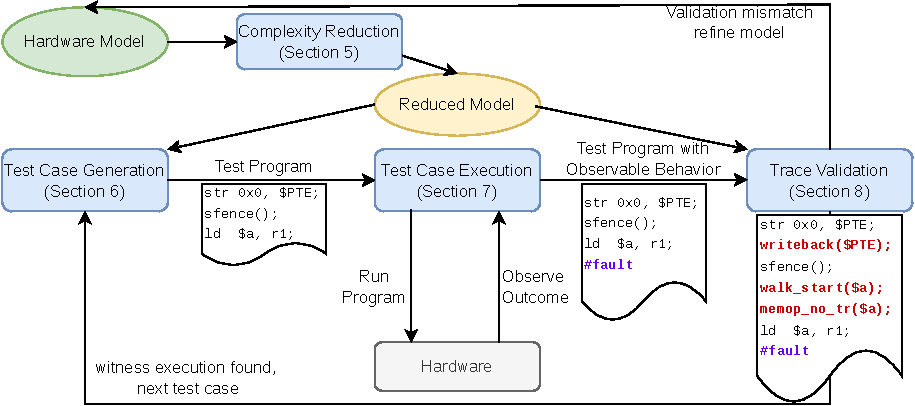
\includegraphics[width=\columnwidth]{figures/SystemOverview.drawio.pdf}
    % TODO refine. 
    \caption{Overview of the validation methodology. The formal model and
    reduction argument constrain both test generation and trace analysis;
    the harness connects stimulus traces to observations on real hardware.
    {\color{red}\textbf{Probably need to make this a bit nicer... maybe include something that hints at the internal steps}}
    }
    \label{fig:validation-pipeline}
\end{figure*}

\noindent\textbf{Hardware Model} 

\noindent\textbf{Model Reduction}

The model is expected to be consistent across variables like the number of cores, virtual addresses, physical addresses, and trace length. However, testing it across every possible value of these variables is impractical, and synthesising hidden steps for long traces causes a state-space explosion that quickly becomes computationally inviable. We therefore propose a number of informal reduction arguments that identify small representative configurations that still seem capable of exposing the behaviours we care about. These are similar in spirit to small-world or small-scope arguments, where behaviours in a large state space are often expected to have small witnesses. The concrete bounds and the per-resource arguments behind them appear in \Cref{sec:reduction}.

\noindent\textbf{Test Case Generation}

The formal model (\Cref{sec:model}) together with our proposed reduction argument (\Cref{sec:reduction}) constrain a test-case generator that emits observable stimulus traces. We chose to automate generation over hand-written litmus tests approaches such as those in~\cite{owens2009x86tso,alglave2011litmus,alglave2014herding}.

 Generate diverse stimulus traces that expose interesting hardware behaviours while staying within bounds. We ensure this by using our reduction arguments to constrain the test case generation process. The generator emits only externally invocable actions such as data memory operations and page table writes, since these are the only events the harness can issue.

\noindent\textbf{Test Execution Harness}

 These stimulus traces are then executed on real hardware via a lightweight harness, producing an observable execution trace including the values returned by data memory operations(reads and writes). 

 Execute each stimulus trace on the hardware under as much isolation as practical, so that the observed read values reflect translation and caching effects in hardware rather than interference from the operating system. 

\noindent\textbf{Trace Validation}

The observable trace is handed to a synthesis-based trace analyser that searches for a sequence of model transitions whose observable projection matches our observed trace. A successful search yields a witness execution (including hidden steps) that explains the observation and counts as a positive validation. A failed search indicates that no model-admissible execution exists for that observation, which is evidence that the model is incorrect or incomplete and can direct improvements. We chose a synthesis encoding of trace checking because the gap between observed and internal traces is exactly the kind of hidden-step reconstruction problem solvers handle well (\Cref{sec:bg:synthesis}).

 Decide whether an observed trace is explainable by the model. We cast this as a synthesis problem such that given the model's transition relation and the observed externals, we try to find a sequence of internal steps that ties them together.
